\documentclass[12pt]{article}

\usepackage{mathtools}
\usepackage{blindtext}

\usepackage[margin=1in]{geometry}

\newcommand*{\eu}{e}
\newcommand*{\iu}{i}

\DeclarePairedDelimiter{\bra}{\langle}{\rvert}
\DeclarePairedDelimiter{\ket}{\lvert}{\rangle}
\DeclarePairedDelimiterX{\braket}[2]{\langle}{\rangle}
  {#1\,\delimsize\vert\,\mathopen{}#2}

\usepackage{biblatex}
\addbibresource{report.bib}

\usepackage[hidelinks]{hyperref}

\title{Solving Decoherence Channels on Open Quantum Systems}
\author{David Basoco \and Jack Hetherington \and Davis Rash \and Tim Ross}
\date{November 8, 2023}

\begin{document}
  \maketitle

  \section{Introduction}
  \blindtext

  \section{Depolarizing and Pauli Channels}
  \blindtext

  \section{Markovian Reservoir Engineering}
  \blindtext

  \section{Amplitude Damping}
  \blindtext

  \section{Results (Applications, Too, or in Another Section)}
  \blindtext

  \begin{figure}
    \centering
    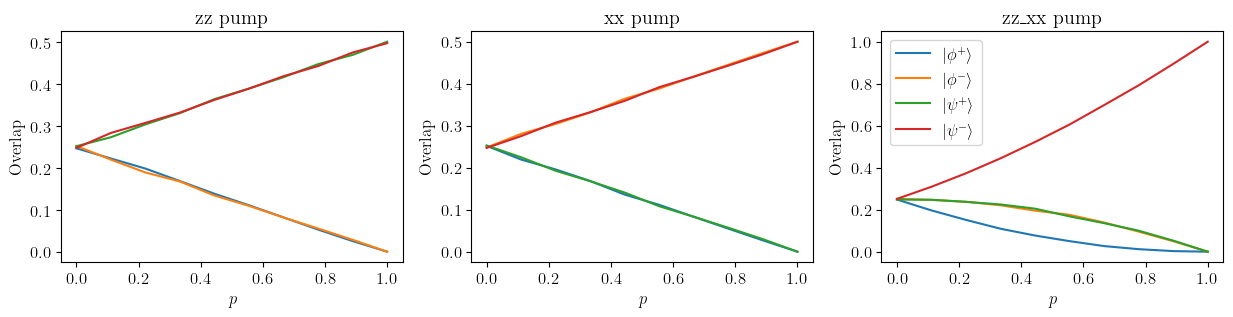
\includegraphics[width=\textwidth]{images/reservoir-engineering-simulation}
    \caption{Simulation of a quantum circuit.%
      \label{fig:reservoir-engineering-simulation}}
  \end{figure}

  \printbibliography
\end{document}